% Document Setup
\documentclass{article}
\usepackage[english]{babel}
\usepackage[letterpaper,top=1.5cm,bottom=1.5cm,left=1.5cm,right=1.5cm,marginparwidth=1cm]{geometry}
\title{Fall 2026 CS4641/CS7641 Homework 1}
\author{Dr. Mahdi Roozbahani\hspace{1cm}Dr. Nimisha Roy\hspace{1cm}Dr. Rodrigo Borela Valente}
\date{Deadline: September 25th, 11:59 pm ET}
\setlength\parindent{0pt}
% end Document Setup



% Common Packages
% """ These are a few packages that may be generally useful (and those used in the typesetting of the questions).
% """ If you find them cumbersome/conflicting with your preferred tools, you may remove them, but this may damage the rendering of some questions, and you are responsible for ensuring you don't misread a question due to a rendering failure.
\usepackage{amsmath, amssymb, marvosym, bbold, bm, mathtools, xfrac} % math symbols
\usepackage{array, multirow} % tables and matrices
\usepackage{enumitem} % dynamic enumeration
\usepackage{graphicx, float} % useful image inclusion
\usepackage{ulem} % underlining
\usepackage{tikz, pgfplots} % great for custom in-line figures, graphs, etc.
\pgfplotsset{compat=1.18}
\usepackage{xparse} % used for our custom linking

% This is what we use to generate content boxes, you're welcome to use it in your solutions.
\usepackage[most]{tcolorbox}
\newtcolorbox{solutionbox}[1][]{
    enhanced, enhanced jigsaw, breakable, colback=gray!10, colframe=gray!40, coltitle=black, arc=4pt, boxrule=0.5pt, boxsep=4pt, left=8pt, right=8pt, top=12pt, bottom=10pt, fonttitle=\bfseries, title=Solution, attach boxed title to top left={yshift=-2mm, xshift=3mm}, boxed title style={colback=gray!40, colframe=gray!60, sharp corners}, #1
} % To make one of these boxes, just do \begin{solutionbox} or \begin{solutionbox}[optional argument override]
\newtcolorbox{hintbox}[1][]{
    enhanced, enhanced jigsaw, breakable, colback=blue!10, colframe=blue!40, coltitle=black, arc=4pt, boxrule=0.5pt, boxsep=4pt, left=8pt, right=8pt, top=12pt, bottom=10pt, fonttitle=\bfseries, title=Hint, attach boxed title to top left={yshift=-2mm, xshift=3mm}, boxed title style={colback=blue!30, colframe=blue!50, sharp corners}, #1
} % We use these to supply hints.
\newtcolorbox{warningbox}[1][]{ 
    enhanced, enhanced jigsaw, breakable, colback=red!10, colframe=red!40, coltitle=black, arc=4pt, boxrule=0.5pt, boxsep=4pt, left=8pt, right=8pt, top=12pt, bottom=10pt, fonttitle=\bfseries, title=Warning, attach boxed title to top left={yshift=-2mm, xshift=3mm}, boxed title style={colback=red!30, colframe=red!50, sharp corners}, #1
} % We use these to note grading directives.
\allowdisplaybreaks

% This is what we use to generate nice-looking links and hypertext references.
\usepackage{hyperref}
\hypersetup{colorlinks=true, linkcolor=blue, filecolor=magenta, urlcolor=cyan, pdftitle={Sharelatex Example}, pdfpagemode=FullScreen}
\definecolor{TODO}{RGB}{180,0,0}
\definecolor{done}{RGB}{0,0,238}
\NewDocumentCommand{\link}{v m}{\href{#1}{\textcolor{done}{\uline{#2}}}}
\NewDocumentCommand{\reviewlink}{v m}{\href{#1}{\textcolor{TODO}{\uline{#2}}}}
% To make one of these links, just do \link{myUrl.com}{displayed text}
% end Common Packages



% Custom Commands
\newcommand{\prob}{\mathbb{P}}
\DeclareMathOperator{\tr}{tr}
% end Custom Commands



% Your Packages
% """ You can use any package you'd like to format your solutions!
% """ We don't mind what your LaTeX looks like, only that it's readable in its final render.
%\usepackage{whateveryouwant}
% end Your Packages



% Rendering
% """ The physical rendering of the document begins here!
% """ To add rendered content, you may write anywhere below \begin{document}.
% """ You may also add content in the provided files that are included with \input below.
% """ You're also welcome to add your own solution files. Any way you want to render your solution is permissible, so long as it adheres to the guidelines in the instructions.
\begin{document}

\maketitle
\begin{itemize}
    \itemsep0.1em
    \item No unapproved extension of the deadline is allowed. Refer to the syllabus for the late submission policy.
    \item Any section marked ``Bonus for Undergrads'' is optional extra credit for undergrads, but is \textbf{required for graduate students!} Any section marked ``Bonus for All'' is optional extra credit for everyone.
    \item \textcolor{red}{Poorly formatted work may disrupt grading and may result in a \textbf{0 on affected questions}.} See ``Completing the Assignment'' in the instructions below for more details.
    \item \textcolor{red}{On most questions, work is required. Failure to show your work when expected may result in a \textbf{0 on affected questions}.} See ``Showing your Work'' in the instructions below for more details.
    \item \textcolor{red}{Failure to properly assign pages in Gradescope may disrupt grading and may result in a \textbf{0 on affected questions}.} See ``Submitting your Work'' in the instructions below for more details.
    \item Discussion is encouraged! You are welcome to discuss at a whiteboard level with peers, but each student must write their own answers and explicitly mention any high-level collaborators. \textcolor{red}{Plagiarism is a \textbf{serious offense}.} You are not allowed to copy and paste, or paraphrase, or submit materials created or published by others, as if you created the materials. A good heuristic for cooperation is to discuss the questions together without discussing specifics, then write up your work and conclusions separately. If a conversation with a peer was meaningfully useful, please add their name to the Collaborators list below.
    \item \textcolor{red}{Working with a generative-AI platform \textbf{may constitute plagiarism}.} In line with the Joyner Heuristic being used by many classes at GT, you should treat collaboration with generative-AI as collaboration with a knowledgeable peer. It would be appropriate to ask about topics and formulae, but inappropriate to share the question and ask them to solve it. \textbf{Sharing the question or your work verbatim with an AI agent so as to generate an answer to the question is considered academic dishonesty and will be treated the same as any other incident of academic dishonesty.} If you're stuck, make a post on Ed, or visit office hours!
    \item \textcolor{red}{Even using generative-AI for formatting your answers is \textbf{not permitted}.} While we understand that \LaTeX~has a learning curve, you may not use any generative-AI platform to improve your writing or \LaTeX~formatting. These tools inherently produce output that may include a partial or complete solution to the question, including corrections to work you give it, even if purely prompted for syntactic use. Additionally, you have no custody over the data you give these platforms, which may leak or be used to inform subsequent training. Thus, while you are more than welcome to ask it about \LaTeX~commands and formatting tips, \textbf{sharing the question or your answer to a question verbatim with an AI agent, even purely for syntactic use, is considered academic dishonesty and will be treated the same as any other incident of academic dishonesty.} If you need formatting help, make a post on Ed, or visit office hours!
    \item \textcolor{red}{All incidents of suspected dishonesty, plagiarism, or violations of the Georgia Tech Honor Code will be subject to the institute's Academic Integrity procedures. If we observe any (even small) issues detected by Gradescope or our TAs, \textbf{WE WILL DIRECTLY REPORT ALL CASES TO OSI}, which may, unfortunately, lead to a very harsh outcome, for example, academic probation or dismissal, a 0 grade for assignments concerned, and prohibition from withdrawing from the class.}
\end{itemize}

\textbf{Collaborators:} \textit{Please include whiteboard-level collaborators here, if any.}
\newpage

\section*{Instructions}
\subsection*{Completing the Assignment}
\begin{itemize}
    \item We provide you the source .tex files that contain the questions. We recommend completing the non-programming part of the assignment in a \LaTeX~editor. The ability to use \LaTeX~is a valuable skill in academia and in industry, and it's generally a clean way to render complicated math. Make sure that your work is formatted correctly. For example, you must submit $\sum_{i=0} x_i$ instead of \text{sum\_\{i=0\} x\_i}.
    \item You may use any \LaTeX~rendering tool you like! \link{https://www.overleaf.com/}{Overleaf} is a great tool, with very few limitations. However, if you want finer control over packages and faster rendering, you may want to download a TeX distribution, a perl binary (if you're on Windows), and the ``Latex Workshop'' extension in VSCode to get live rendering in VSCode.
    \item If you're uncomfortable with using \LaTeX, no worries! You can simply use the pdf version of the non-programming assignment and build your answers in any word or markdown processor you prefer. However, there are some caveats:\begin{enumerate}[label = \arabic*.]
        \item \textbf{We will \underline{NOT} grade handwritten work.} You must use some digital processor to render your work into a cleanly formatted pdf.
        \item It is \textbf{your responsibility} to ensure the questions are correctly numbered. While we will attempt to grade your work accurately, misnumbering may cause misinterpretation.
        \item It is \textbf{your responsibility} to ensure you're answering the question as it is written. We find that students who work without the questions embedded in their document tend to misinterpret the question more often. If you work in a separate document, read carefully and consider copying over the source question, even if its formatting may be lost.
    \end{enumerate}
\end{itemize}
\subsection*{Showing your Work}
\begin{itemize}
    \item When a question asks you to \emph{show your work}, you must provide a justification for your solution. This may include calculations or text-based explanation. Though basic arithmetic may be combined, your work should be thorough and clear enough for a reader to follow your line of reasoning.
    \item When a question asks you to \emph{prove} or \emph{provide a proof of} some statement, you must provide a formal proof. These questions have a higher burden of work, and must constitute a valid inference. Again, while basic arithmetic can be combined, your work should be defensible as a formal proof. Any gaps in logic or unstated assumptions may result in deductions. Be careful using identities you may find online, since they may assume the fact you are trying to prove.
    \item If not otherwise indicated, no justification is needed, just the final answer.
    \item You will never be penalized for showing too much work, but you may be penalized for not showing enough.
    \item If you use an online resource, please cite it. We generally permit most resources, and so, citing it will only be to your benefit in the case of a plagiarism investigation (in the common case where multiple students utilize the same source).
\end{itemize}
\subsection*{Submitting your Work}
\begin{itemize}
    \item We will be using Gradescope for submission and grading of assignments. Complete the assignment, convert your assignment to a pdf, and submit it to the appropriate assignment denoted ``Non-Programming'' on Gradescope.
    \item When submitting your assignment on Gradescope, you are required to map pages of your pdf to subquestions on the homework. You should select a subquestion, then map it to \textbf{every} page which contains any portion of your solution to that subquestion.
    \item \textbf{You must map every page on which you have content that you would like be graded.} During the grading of each particular subquestion, we only see the pages you assign to that subquestion, so you must assign everything you would like us to grade.
    \item \textbf{Improperly mapped questions will receive penalties, up to and including 0 credit for the question.} You are permitted to submit a regrade request in this event; however, the review of such a request is at the sole discretion of the instructional staff and is not likely to be accepted.
    \item Some tips to correctly assign pages:
    \begin{enumerate}[label = \arabic*.]
        \item Underassigning pages is a common mistake. For example, if your answer to question 4.2 starts halfway down on page 16, goes through page 17, and ends with a single line bleeding into page 18, assign pages 16, 17, \textit{and} 18 to question 4.2. Assigning just page 16 may incur a page assignment penalty, or the grader may just interpret your work as incomplete.
        \item Keep in mind that overassigning is just as slowing to the grading process as underassigning is. Please try to keep your assignments tight around the content for the specific subquestion. E.g., assigning every page is just as useless as assigning no pages.
    \end{enumerate}
    \textbf{Again, assign every page that has content relevant to your answer that you would like for us to see while grading. If you don't assign it, we can't see it.}
\end{itemize}
\newpage

\section*{Point Distribution}
\subsection*{Q1: Linear Algebra [21pts]}
\begin{enumerate}[label=\arabic*.]
    \itemsep0em
    \item More General Inner Products [9pts]
    \item More General Norms [6pts]
    \item Eigen-stuff [6pts]
\end{enumerate}

\subsection*{Q2: Working with Markov Chains [18pts Grad / 6\% Bonus for Undergrads]}
\begin{enumerate}[label=\arabic*.]
    \itemsep0em
    \item Markov Mechanics [6pts Grad / 2\% Bonus for Undergrads]
    \item Application to PageRank [12pts Grad / 4\% Bonus for Undergrads]
\end{enumerate}

\subsection*{Q3: Probability and Statistics [30pts]}
\begin{enumerate}[label=\arabic*.]
    \itemsep0em
    \item Joint Distributions and Independence [6pts]
    \item Covariance and Correlation [8pts]
    \item Gaussian Distributions [6pts]
    \item Conceptual Questions and Proofs [10pts]
\end{enumerate}

\subsection*{Q4: Parameter Estimation Challenge [10pts]}

\subsection*{Q5: Optimization [15pts + 6\% Bonus for All]}
\begin{enumerate}[label=\arabic*.]
    \itemsep0em
    \item KKT Conditions [15pts + 2\% Bonus for All]
    \item Using Jensen's for Convexity [4\% Bonus for All]
\end{enumerate}

\subsection*{Q6: Information Theory [35pts]}
\begin{enumerate}[label=\arabic*.]
    \itemsep0em
    \item Entropy Proofs [20pts]
    \item KL-Divergence [5pts]
    \item Entropy and Informativity [10pts]
\end{enumerate}

\subsection*{Q7: Entropy Bound [4\% Bonus for All]}

\bigskip
\subsection*{Points Totals:}
\begin{itemize}
    \item Non-Programming Base:\begin{itemize}
        \itemsep0em
        \item Undergrad: 111 pts
        \item Graduate: 129 pts
    \end{itemize}
    \item Non-Programming Bonus for Undergrad:\begin{itemize}
        \itemsep0em
        \item Undergrad: 6\%
        \item Graduate: these questions are required and included as base points
    \end{itemize}
    \item Non-Programming Bonus for All:\begin{itemize}
        \itemsep0em
        \item Undergrad: 10\%
        \item Graduate: 10\%
    \end{itemize}
    \item For programming related points, see the Jupyter notebook.
\end{itemize}

\newpage
\section{Linear Algebra [20pts]}



\subsection{More General Inner Products [9pts]}
In lecture, we will have discussed a lot of properties of the dot product on $\mathbb{R}^n$. The dot product is a prolific example of a more general operation: an \textbf{inner product}. There are many ways you could formulate an inner product on $\mathbb{R}^n$. An inner product is typically denoted as $\langle \cdot, \cdot\rangle$, and just needs to satisfy a number of axioms.\footnote{For $\mathbb{R}^n$, generally, we look for Symmetry ($\forall\vec{x},\vec{y};\;\; \langle \vec{x}, \vec{y}\rangle = \langle \vec{y}, \vec{x}\rangle$), Linearity in the First Argument ($\forall\vec{x},\vec{y},\vec{z},\alpha\in\mathbb{R},\beta\in\mathbb{R};\;\; \langle \alpha\vec{x} + \beta \vec{y}, \vec{z}\rangle = \alpha\langle \vec{x}, \vec{z}\rangle + \beta\langle \vec{y}, \vec{z}\rangle$), and Positive-Definiteness ($\forall\vec{x};\;\; \langle\vec{x}, \vec{x}\rangle = 0 \iff \vec{x} = \vec{0}$, and $\forall\vec{x};\;\; \langle \vec{x}, \vec{x} \rangle \geq 0$).}

\smallskip Different inner products give us different conceptualizations of \textit{angles} between vectors. More specifically, a pair of vectors $\vec{x}, \vec{y}$ are said to be \textbf{orthogonal} if and only $\langle \vec{x}, \vec{y}\rangle = 0$. However, since the inner product is a broad category of functions, it is very possible for two vectors to be orthogonal with respect to some inner product not orthogonal with respect to another.

\smallskip Consider the following vector.
$$\vec{v}=\begin{bmatrix}1 \\ 1 \\ 3\end{bmatrix}$$
For each of the following inner products, you must find the \emph{set of all vectors} orthogonal to $\vec{v}$ under that inner product. \emph{Show your work.} [3pts each]

\begin{enumerate}[label=\alph*.]
    \item $\langle (x_1, x_2, x_3), (y_1, y_2, y_3) \rangle_a \;\coloneq\; x_1y_1 + x_2y_2 + x_3y_3$ 
    \item $\langle (x_1, x_2, x_3), (y_1, y_2, y_3) \rangle_b \coloneq 9x_1y_1 + 4x_2y_2 + x_3y_3$
    \item $\langle (x_1, x_2, x_3), (y_1, y_2, y_3) \rangle_c \coloneq 6x_1y_1 - 2x_1y_2 - 2x_2y_1 + 3x_2y_2 + 3x_3y_3$
\end{enumerate}

\begin{hintbox}
The set of vectors orthogonal to a given vector is likely to be infinite. In that case, you should parametrize your result. A standard format is set builder notation, which defines sets more generally:

$$\left\{ \text{arbitrary formula to make an element} \;\Big|\; \text{rules for inclusion in the set}\right\}$$

For example, to express the plane $z=0$ of $\mathbb{R}^3$ in set-builder notation, we could say:

$$S = \left\{ a\begin{bmatrix}1 \\ 0 \\ 0\end{bmatrix} + b\begin{bmatrix}0 \\ 1 \\ 0\end{bmatrix} \;\Bigg|\; \forall a,b\in\mathbb{R}\right\}$$

You do not need to use this particular notation. You may solve the question however you like, and you may express your answer however you like, but you must parametrize your result such that you appropriately express the set of all vectors orthogonal to $\vec{v}$.
\end{hintbox}

\newpage



\subsection{More General Norms [6pts]}
In lecture, we will have discussed a lot of properties of the $L_1$ and $L_2$ norms. You may have also heard those called Manhattan and Euclidean distance, respectively. These distance functions are prolific examples of a more general operation: a \textbf{norm}.

Just like we can define any number of different inner products to explore different conceptualizations of \textit{vector angles}, we can also define new norms to explore different conceptualizations of \textit{vector distance/length}. A norm is any function that maps a vector space to the non-negative real numbers. However, recall from lecture that it must also satisfy three properties: positive-definiteness, absolute homogeneity, and triangle inequality/subadditivity (check the lecture slides for more precise formulations).

Then, for each of the following functions: [2pts each]
\begin{itemize}
    \itemsep 0em
    \item if they \textit{do not} constitute a valid norm, you may merely \emph{indicate} one property of norms they violate and provide an example input where the function violates that property.
    \item if they \textit{do} constitute a valid norm, you must \emph{prove} that they satisfy all three properties of norms mentioned above.
\end{itemize}

\begin{enumerate}[label=\alph*.]
    \item $f \colon \mathbb{R}^2 \to \mathbb{R}_{\ge 0}$ with
        $$f((x_1, x_2)) = \biggl|\sin(x_1^2) + \frac{x_1 + 1}{\sqrt{3}} + 6x_1\biggr| + \biggl|\sin(x_2^2) + \frac{x_2 + 1}{\sqrt{3}} + 6x_2\biggr|$$
    \item $g \colon \mathbb{R}^2 \to \mathbb{R}_{\ge 0}$ with
        $$g((x_1, x_2)) = \sqrt{|x_1|^2 + |x_2|^{4}}$$
    \item $h \colon \mathbb{R}^{3} \to \mathbb{R}_{\ge 0}$ with
        $$h((x_1, x_2, x_3)) = |x_1| + 3|x_2| + 6|x_3|$$
\end{enumerate}

\begin{hintbox}
Proving positive-definiteness, absolute homogeneity, and triangle inequality/subadditivity from scratch can be a bit tricky. It helps to work from existing functions that you already know are norms.

\smallskip These functions all make use of the absolute value function $|x|$. You may safely assume that this is a valid norm on $\mathbb{R} \to \mathbb{R}_{\ge 0}$ (as though the input were a 1-D vector space). Thus, it will satisfy the three properties—positive-definiteness, absolute homogeneity, and triangle inequality/subadditivity. You may invoke this in your proofs as a given wherever necessary.
\end{hintbox}
\newpage



\subsection{Eigen-stuff [6pts]}
\begin{enumerate}[label=\alph*.]
    \item Given the following matrix $\boldsymbol{A}$, solve for its eigenvalues ($\lambda_1, \lambda_2$) in terms of $a$, $b$, and $c$. \emph{Show your work.} [3pts]

    $$\boldsymbol{A}=\begin{bmatrix}
        a & b \\
        b & c
    \end{bmatrix}$$

    \item Let $\boldsymbol{B}$ be a real-valued, symmetric, $3 \times 3$ matrix. $\vec{v}_1$ and $\vec{v}_2$ are eigenvectors of $\boldsymbol{B}$ that correspond to real, distinct eigenvalues $\lambda_1, \lambda_2$; they are as follows:
    $$\vec{v}_1 = \begin{bmatrix}1 \\ 2 \\ 1\end{bmatrix} \qquad \vec{v}_2 = \begin{bmatrix}-2 \\ 1 \\ 0\end{bmatrix}$$
    Suppose that $B$ has one more eigenvalue $\lambda_3$ that's different from the other 2. Find the third eigenvector, a non-zero vector $\vec{v}_3 \in \mathbb{R}^3$, such that $\boldsymbol{B}\vec{v}_3 = \lambda_3\vec{v}_3$, and $\lambda_3 \neq \lambda_2, \lambda_3 \neq \lambda_1$. \emph{Show your work.} [3pts]

    \begin{hintbox}

        This would be very difficult to deduce for a general matrix $\boldsymbol{B}$, but we have that $\boldsymbol{B}$ is a real-valued, symmetric matrix. What, then, can we conclude about its eigenvectors? (the answer is in the slides...)
    \end{hintbox}
\end{enumerate}
\newpage


\newpage
\section{Working with Markov Chains [18pts Grad / 6\% Bonus for Undergrads]}



\subsection{Markov Mechanics [6pts Grad / 2\% Bonus for Undergrads]}
Suppose we have a sequence of random variables $\{X_t\}_{t \in \mathbb{Z}^{\ge 0}}$ that take on values from the set $\mathcal{S} \coloneq \{1, 2, \dots, n\}$ (where $n$ is just some positive integer). We could think of the value of $X_t$ as the state of some system at time $t$ and we could think of $\mathcal{S}$ as the set of all possible states the system could be in. Naturally, we'd like to compute $P(X_t = x_t)$, the probability that the system is at state $x_t \in \mathcal{S}$ at time $t$. If we make the assumption that this is modelling a physical system, we can conclude the current state is dependent on the past, but not on the future. Furthermore, we suppose the system can take any value from $\mathcal{S}$ at every time $t$. Thus, we can say:
\begin{equation} \label{eq:longeq}
    P(X_t = x_t) = \sum_{x_{t - 1} \in \mathcal{S}}\sum_{x_{t - 2} \in \mathcal{S}} \dots \sum_{x_{0} \in \mathcal{S}}P(X_t = x_t \mid X_{t - 1} = x_{t - 1}, \dots, X_0 = x_0)P(X_{t - 1} = x_{t - 1}, \dots, X_0 = x_0).
\end{equation}
As it stands now, computing $P(X_t = x_t)$ for a fixed $x_t$ would require us to add $n^t$ terms and know all of the different $n^t$ conditional probability distributions, which becomes intractible for relatively small values of $n$ and $t$. To simplify, we can make an assumption known as the \textbf{first-order Markov assumption}:
$$P(X_t = x_t \mid X_0 = x_0, \dots, X_{t - 1} = x_{t - 1}) = P(X_t = x_t \mid X_{t - 1} = x_{t - 1}),$$
for any $t \geq 1$. We've assumed that the current state is dependent only on the most recent state, and not the entire history. Our sequence $\{X_t\}_{t \in \mathbb{N}}$ is now called a \textbf{Markov chain}. You can verify that \eqref{eq:longeq}, under this assumption, becomes
$$P(X_t = x_t) = \sum_{x_{t - 1} \in S} P(X_t = x_t \mid X_{t - 1} = x_{t - 1})P(X_{t - 1} = x_{t - 1}).$$
With this assumption, we only need to know the conditional probabilities for a single timestep, $P(X_{t} = i \mid X_{t - 1} = j)$ for all $i, j \in \mathcal{S}$, and the distribution over the initial states, $P(X_0 = x_0)$ for any $x_0 \in \mathcal{S}$. These conditional probabilities are known as \textbf{transition probabilities}. It's also common to model these transition probabilities as constant over time, that is, $P(X_{t} = i \mid X_{t - 1} = j) = P(X_{q} = i \mid X_{q - 1} = j)$ for any $q, t \geq 1$ and $i, j \in \mathcal{S}$. To organize the transition probabilities, we can define a matrix $A \in \mathbb{R}^{n \times n}$ such that $A_{ij} \coloneq P(X_{t} = i \mid X_{t - 1} = j)$\footnote{You'll have to use 1-indexing if you want this to align with our definition $\mathcal{S} \coloneq \{1, 2, \dots, n\}$.}. Because these are probabilities over all $\mathcal{S}$, all entries will be non-negative, and the columns will sum to 1:
$$ \forall j \; \left[ \sum_{k = 1}^n A_{kj} = 1 \right] \qquad \text{and} \qquad \forall i,j\; \left[ A_{ij} \geq 0 \right] $$
Matrices with these properties are called \textbf{stochastic matrices}. If we let $\vec{x}_0 \coloneq \begin{bmatrix}P(X_0 = 1) & \dots & P(X_0 = n)\end{bmatrix}^\top$, we can simulate a time-evolution of the system simply by multiplying by the matrix, $\vec{x_1}=A\vec{x_0}$\footnote{It may be instructive to work out a single element of $\vec{x_1}$ symbolically, and confirm that it does correctly evaluate the sum rule using the transition probabilities to get the probability of the system at the next timestep.}. More generally, the $i$-th entry of $\vec{x}_t \coloneq A\vec{x}_{t - 1}$ is $P(X_t = i)$. Crucially, since we assumed that the transition probabilities are constant over time, we don't even need a recurrence relation, we can just repeatedly multiply $\vec{x_0}$ by $A$, $\vec{x}_t = A^t\vec{x}_0$.

\begin{enumerate}[label=\alph*.]
    \item Given an $n \times n$ stochastic matrix $A$, \emph{prove} that 1 is always an eigenvalue of $A$. [3pts Grad / 1\% Bonus for Undergrads]

    \item Let's interpret that result. Given an eigenvalue $\lambda$ of $A$, we know that there must exist an eigenvector $\vec{v}$ such that $A\vec{v} = \lambda\vec{v}$. With $\lambda=1$, we know further that $A\vec{v}=\vec{v}$. Interpreting $A$ as a transformation, $\vec{v}$ is unaffected by this transformation. When such a $\vec{v}$ is a \textit{probability vector} (i.e., a vector whose entries are non-negative and sum to 1), then interpreting $\vec{v}$ as a distribution over our states $\mathcal{S}$ means that this distribution over the states is unaffected by time-evolution. Thus, it's called a \textit{steady-state vector}. When the state of our system has approached a steady-state vector with $A\vec{v}=\vec{v}$, then our belief of the state of the system doesn't change.

    \smallskip Given the stochastic matrix $$A = \begin{bmatrix}1/2 & 2/3 \\ 1/2 & 1/3\end{bmatrix},$$
    find all steady-state vectors of the corresponding Markov chain. Remember to normalize your result to a probability vector. \emph{Show your work. Round your final result to 3 decimal places.} [3pts Grad / 1\% Bonus for Undergrads]
\end{enumerate}
\newpage



\subsection{Application to PageRank [12pts Grad / 4\% Bonus for Undergrads]}
The Google PageRank algorithm is a classic application of Markov chains. The main objective is ranking webpages by their importance, which we roughly take to mean the proportion of time a user spends on a webpage as they surf the Web. Each webpage is a state, and the transition probabilities dictate how a user moves between the webpages that are hyperlinked on the current webpage. To satisfy some regularity conditions, slight adjustments are made to the stochastic matrix $A$ (i.e., the final stochastic matrix we get isn't going to only be made up of the transition probabilities as was explained in the previous part):

\begin{itemize}
    \itemsep0em
    \item If there exists a column of $A$ with only a single entry being 1, replace the whole column of $A$ with $1/n$, where $n$ is the number of webpages in total, to get a new matrix $A'$.
    
    \item We then compute the Google matrix $G$, where
    $$G \coloneq \alpha A' + (1 - \alpha)K,$$
    $0 < \alpha < 1$, and $K$ is the matrix with all entries equal to $1/n$. The idea is that sometimes a websurfer will close the tab and start a new search at a random site.
    
    \item $G$ is the stochastic matrix that represents an appropriate Markov chain for modelling our problem. 
\end{itemize}
Now, $G$ must have a unique steady state $\vec{x}^*$, that is, for any valid initial distribution $\vec{x}_0$, we have that
$$\vec{x}^* \coloneq \lim_{k \to \infty} \vec{x}_k = \lim_{k \to \infty} G^k\vec{x}_0 \implies G\vec{x}^* = \vec{x}^*$$

Suppose we have 3 webpages on the Web. The following graph represents the different transition probabilities between the webpages.

\begin{figure}[!h]
    \centering
    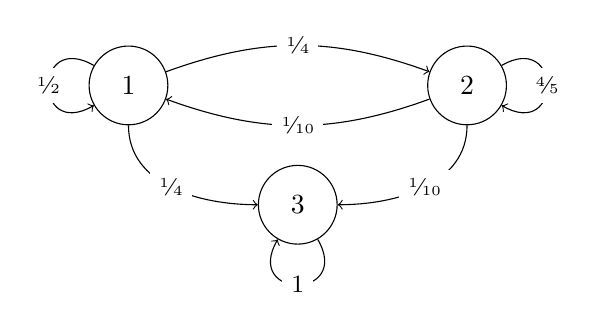
\begin{tikzpicture}[thin, node distance=43mm, main/.style = {draw, circle, minimum size=1cm}, lbl/.style={midway, fill=white, font=\small}]
        \node[main] (1) {$1$};
        \node[main] (2) [right of=1] {$2$};
        \draw[bend left=20, ->] (1) to node[lbl] {\sfrac{1}{4}} (2);
        \draw[bend left=20, ->] (2) to node[main] (3) [midway, below=0.5cm] {$3$} node[lbl] {\sfrac{1}{10}} (1);
        \draw[->] (1) to [out=150, in=210, looseness=4.5] node[lbl] {\sfrac{1}{2}} (1);
        \draw[->] (2) to [out=30, in=330, looseness=4.5] node[lbl] {\sfrac{4}{5}} (2);
        \draw[->] (1) to [out=270, in=180] node[lbl] {\sfrac{1}{4}} (3);
        \draw[->] (2) to [out=270, in=0] node[lbl] {\sfrac{1}{10}} (3);
        \draw[->] (3) to [out=300, in=240, looseness=4.5] node[lbl] {1} (3);
    \end{tikzpicture}
\end{figure}

For the sake of cleanliness, we've excluded any edges with a weight of 0, but all other edges should be present and interpretable as transition probabilities. For example, we see here that $P(X_{t} = 2 \mid X_{t - 1} = 1) = \frac{1}{4}$.

You'll be applying PageRank to this tiny web. From user surveying, we've found that $\alpha=0.8$ is a good choice for our modelling purposes.

\begin{enumerate}[label=\alph*.]
    \item Construct the base stochastic matrix, $A$. [1.5pts Grad / 0.5\% Bonus for Undergrads] % no work required to be shown
    \item Construct $G$. \emph{Show your work.} [6pts Grad / 2\% Bonus for Undergrads]
    \item Find the unique steady-state vector of $G$. \emph{Show your work.} [3pts Grad / 1\% Bonus for Undergrads]
    \item Order the webpages by how frequently a user would visit the webpages as they surf the Web indefinitely. [1.5pts Grad / 0.5\% Bonus for Undergrads] % no work required to be shown
\end{enumerate}
\begin{warningbox}
    Your work will be easier to evaluate if you do not round intermediate results. You should represent all numbers appearing in your work for this question as fractions or integers.
\end{warningbox}
\newpage


\newpage
\section{Probability and Statistics [30pts]}



\subsection{Joint Distributions and Independence [6pts]}
The following table summarizes data collected from 10 students. Let $X$ be a random variable that is $1$ if the student studied for an exam and $0$ otherwise. Let $Y$ be a random variable that is $1$ if the student passed the exam and $0$ otherwise.

\begin{center}
\begin{tabular}{l|cc|r}
\hline\hline
 & $Y=1$ (Passed) & $Y=0$ (Failed) & Total \\
\hline
$X=1$ (Studied) & 4 & 2 & 6 \\
$X=0$ (Didn't Study) & 1 & 3 & 4 \\
\hline
Total & 5 & 5 & 10 \\
\hline\hline
\end{tabular}
\end{center}

Answer the following questions using the empirical data about $X$ and $Y$ in the table above.

\begin{enumerate}[label=\alph*.]
    \item Compute $P(X=1, Y=1)$. \emph{Round your final result to 3 decimal places.} [1pts] % no work required to be shown

    \item Compute the marginal probabilities $P(X=1)$ and $P(Y=1)$. \emph{Round your final result to 3 decimal places.} [1.5pts] % no work required to be shown

    \item Compute the conditional probability $P(Y=1 \mid X=1)$. \emph{Round your final result to 3 decimal places.} [1.5pts] % no work required to be shown

    \item Are $X$ and $Y$ statistically independent? \emph{Justify your answer} using your previous calculations. [2pts]
\end{enumerate}
\newpage



\subsection{Covariance and Correlation [8pts]}
\begin{enumerate}[label=\alph*.]
    \item Suppose $X$ and $Y$ are two random variables. $X$ has the pmf:
    $$
    p(x) = \begin{cases} 0.3 & x = c \\ 0.7 & x = -c \end{cases}
    $$
    where $c$ is a nonzero constant. Let $Y$ obey the Standard Normal distribution, $Y \sim \mathcal{N}(0, 1)$.
    
    $X$ and $Y$ are statistically independent. Define a new random variable $Z = X - Y$. Calculate the covariance of $Y$ and $Z$, i.e., $\mathsf{Cov}(Y, Z)$. \emph{Show your work. Round your final result to 3 decimal places.} [5pts]

    \item Let $A$ and $B$ be statistically independent random variables with $\mathsf{Var}(A) = 2$ and $\mathsf{Var}(B) = 15$. Define a new random variable $C = 4A + 2B$. The correlation coefficient, $\rho(A, C)$, is defined as:
    $$
    \rho(A, C) = \frac{\mathsf{Cov}(A, C)}{\sqrt{\mathsf{Var}(A)\,\mathsf{Var}(C)}}
    $$
    Calculate $\rho(A, C)$, the correlation coefficient between $A$ and $C$. \emph{Show your work. Round your final result to 3 decimal places.} [3pts]
\end{enumerate}
\newpage



\subsection{Gaussian Distributions vs. Gaussian-Distributed Random Variables [6pts]}
You are given two \textbf{independent} random variables, $X_1 \sim \mathcal{N}(\mu_1, \sigma_1^2)$ and $X_2 \sim \mathcal{N}(\mu_2, \sigma_2^2)$.
These are ``\textit{Gaussian-distributed random variables},'' that is, their probability density functions are described by the Gaussian function:
$$\mathcal{N}(\mu, \sigma^2)=\frac{1}{\sqrt{2\pi\sigma^2}}\cdot \exp\left( -\frac{(x-\mu)^2}{2\sigma^2} \right)$$

\begin{enumerate}[label=\alph*.]
    \item Let $Y = X_1 + X_2$. One way to conceptualize sampling a value for $Y$ is to imagine sampling a value for both $X_1$ and $X_2$, then adding the results of those trials. Curiously, the probability density function of $Y$ is also a Gaussian. The standard result for $Y = X_1 + X_2$ would be $Y \sim \mathcal{N}(\mu_1 + \mu_2, \sigma_1^2 + \sigma_2^2)$. Proving that $Y$ is actually Gaussian-distributed requires some tools we haven't taught, but a much easier result is to confirm the mean and variance.

    Show that $\mathbb{E}[Y]=\mu_1 + \mu_2$ and $\mathsf{Var}(Y)=\sigma_1^2 + \sigma_2^2$. \emph{Show your work.} [3pts]

    \item Now consider a new random variable $Z$, defined as:
    $$Z = \begin{cases}
        X_1 & \text{with probability } 0.5 \\
        X_2 & \text{with probability } 0.5
    \end{cases}$$
    Can $Z$ be described as a Gaussian random variable? \emph{Briefly (1-2 sentences or quick math) justify} your choice. [3pts]

\end{enumerate}
\newpage



\subsection{Conceptual Questions and Proofs [10pts]}
\begin{enumerate}[label=\alph*.]
    \item Variance is defined as the expected amount by which data varies from the mean.
    $$\mathsf{Var}(X) = \mathbb{E}[(X-\mathbb{E}[X])^2]$$
    You can also formulate variance using only the first- and second-order moments of the random variable.
    $$\mathsf{Var}(X) = \mathbb{E}[X^2] - (\mathbb{E}[X])^2$$

    Using algebra and expectation identities, \emph{prove} that these two formulations are equivalent. [5pts]

    \item \emph{Explain} in your own words why two random variables can be uncorrelated (i.e., $\mathsf{Cov}(A, B)=0$) but also not statistically independent (i.e., $P(A,B)\neq P(A)\cdot P(B)$).
    Also, \emph{provide one simple example} of two random variables that demonstrate this property. [5pts]
\end{enumerate}
\newpage


\newpage
\section{Parameter Estimation Challenge [10pts]}
You're about to play a game of chance, and your opponent provides a coin. They say, ``don't worry, it's a fair coin,'' but because they even thought to say that, now you don't trust them. We can model the coin as a random variable $C$ with a single parameter $\theta\in[0,1]$, the chance of landing on heads.
$$C=\begin{cases}
    \text{Heads} & p=\theta \\
    \text{Tails} & p=1-\theta
\end{cases}$$
If it were a fair coin, we would have $\theta=0.5$, but this is ML, so let's start modelling! Your opponent hands you the coin for you to inspect. There's no obvious visual defects, and, feeling it in your hands, it seems balanced; you don't get the sense that the coin is biased. At this point, `\textit{a priori},' we can model your belief about $\theta$ with the following distribution:

\begin{figure}[htbp]
    \centering
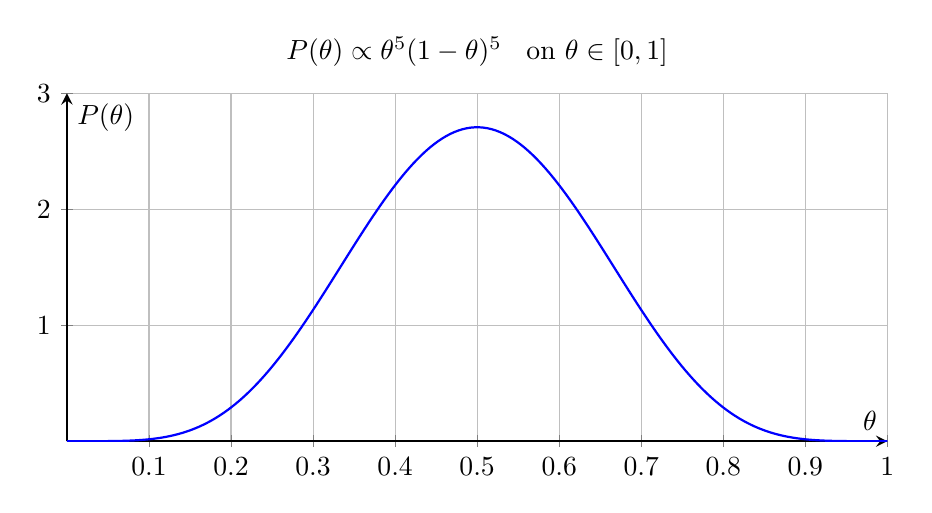
\begin{tikzpicture}
\begin{axis}[
    width=12cm,
    height=6cm,
    xlabel={$\theta$},
    ylabel={$P(\theta)$},
    title={$P(\theta) \propto \theta^5(1-\theta)^5\;\;\text{ on }\theta\in[0,1]$},
    domain=0:1,
    samples=200,
    xmin=0, xmax=1,
    ymin=0, ymax=3,
    axis lines=middle,
    grid=major,
    thick,
]
\addplot[blue, thick] {2772*x^5*(1-x)^5};
\end{axis}
\end{tikzpicture}
\caption{The distribution has a mode at 0.5, but it's not so tight, modelling a healthy distrust of your opponent.}
\end{figure}

We shouldn't rely on touch alone. This choice of `\textit{a priori}' belief may be too generous to your opponent and is frankly unfounded, so let's collect some data. You flip the coin 15 times and get 12 heads and 3 tails (assume these tosses are independent and identically distributed). This isn't promising, but not entirely disqualifying, given the small sample size.

\bigskip In class, you will have learned about Maximum Likelihood Estimation (MLE). You recorded some data, $D$: 12 heads and 3 tails, and you could pick a $\theta$ that maximizes the likelihood of that data, i.e., $\theta^*_{MLE} \coloneq \arg\max_\theta P(D \mid \theta)$. However, this doesn't take into account any prior belief. We need a way to include your prior probability distribution.

\bigskip The more general formulation is \textit{Maximum A Posteriori} (MAP) estimation:

\begin{gather*}
    \mathllap{\theta^*_{MAP}} \coloneq \mathrlap{\arg\max_\theta P(\theta \mid D)} \\
    P(\theta | D)\text{ is the posterior probability, which we can expand with Bayes's Rule} \\
    \mathllap{\theta^*_{MAP}} = \mathrlap{\arg\max_\theta \frac{P(D \mid \theta)\cdot P(\theta)}{P(D)}} \\
    \text{$P(D)$ is the probability of the data, which would be tough to ascertain,} \\
    \text{but it's constant for all $\theta$, so it won't affect the argmax computation} \\
    \mathllap{\theta^*_{MAP}} = \mathrlap{\arg\max_\theta P(D \mid \theta)\cdot P(\theta)}
\end{gather*}
\begin{hintbox}
    Note that we don't actually have our prior $P(\theta)$. There's a proportionality constant required to make it a real pdf (integrates to 1), but—again—since we're taking an argmax, we can drop the proportionality constant as well.

\end{hintbox}

Given our prior belief $P(\theta)$ and our data $D$, formulate the likelihood $P(D\mid\theta)$, then compute the new best estimator, $\theta^*_{MAP}$. \emph{Show your work. Round your final result to 3 decimal places.} [10pts]


\newpage
\section{Optimization [15pts + 6\% Bonus for All]}
\subsection{KKT Conditions [15pts + 2\% Bonus for All]}
Optimization problems are related to minimizing a function (usually termed loss, cost, or error function) or maximizing a function (such as the likelihood) with respect to some variable $x$. The Karush-Kuhn-Tucker (KKT) conditions are first-order conditions for a solution in nonlinear programming to be optimal, provided that some regularity conditions are satisfied. You will learn about the KKT procedure in class, but there is also an example problem in the appendix.

In this question, you will be solving the following optimization problem:
\begin{align*}
    \min_{\vec{x} \in \mathbb{R}^3} \qquad & f(\vec{x}) = 3x_1^2 + 5x_2^2 - x_2x_3 + 2x_3^2, \qquad \vec{x} = (x_1,x_2,x_3) \\
    \text{s.t.} \qquad & g_1(\vec{x}) : x_1 + x_2 + x_3 \leq -4 \\
    & g_2(\vec{x}) : 4x_1^2 \leq 5 \\
    & g_3(\vec{x}) : 3x_2 + 8x_1 \leq -50 \\
    & g_4(\vec{x}) : -x_3^2 \leq -6 \\
\end{align*}

\begin{enumerate}[label=\alph*.]
    \item Write the Lagrange function, $\mathcal{L}(\vec{x}; \lambda_1, \lambda_2, \lambda_3, \lambda_4)$ for this minimization problem. [3pts] % no work required

    \item List the names of all 4 groups of KKT conditions and all their corresponding mathematical equations or inequalities for this specific minimization problem. \emph{Show your work.} [9pts]

    \item Inequality constraints are tough to deal with. In addition to the Lagrange multipliers, KKT introduces the idea of constraint activity. When enumerating all possible constraint activity sets, how many systems would we need to solve? [3pts] % no work required

    \item Find the constrained global minimum! This is quite a lot of work and we don't expect you to do it by hand; you may use any tool you like. Once you set activity, KKT reduces to a system of equalities (and you check the solutions for feasibility after solving), so any tool for solving equations would work.

    \smallskip There are several capable python packages, including \link{https://docs.sympy.org/latest/modules/solvers/solvers.html}{SymPy} or \link{https://doc.sagemath.org/html/en/tutorial/tour_algebra.html#solving-equations-exactly}{sagemath}. There may be online tools, but those tend to be quite limited, especially in the number of variables allowed.

    \smallskip List out all feasible candidates (including their Lagrange multipliers), then perform the candidates test to pick the optimal candidate. \emph{Round your final result to 3 decimal places.} [2\% Bonus for All]
\end{enumerate}


\newpage
\subsection*{Example: Using Jensen's Inequality for Gibbs' Inequality [0pts]}
Jensen's inequality is a very powerful tool in ML. In general,
$$\begin{cases}
    \mathbb{E}\left[f(X)\right] \geq f\left(\mathbb{E}[X]\right) & \text{ when f is convex} \\
    \mathbb{E}\left[f(X)\right] \leq f\left(\mathbb{E}[X]\right) & \text{ when f is concave}
\end{cases}$$
Choosing the right composition function $f$ can generate very useful results. For example, one can use Jensen's inequality to prove Gibbs' inequality, that is, that KL-Divergence is non-negative. For discrete probability distributions $P$ and $Q$,
$$ D_{\text{KL}}(P\|Q) = \sum_i p_i \log\frac{p_i}{q_i} $$
We can express this as an expectation of $\log\frac{p_i}{q_i}$ over the weights $p_i$, which must sum to 1, as they're valid probabilities. For Jensen's we also need a convex function to get $D_{\text{KL}}\geq\cdots$ and not $D_{\text{KL}}\leq\cdots$; log is concave, but then $-\log$ is convex, and that's just a log rule away.
$$ D_{\text{KL}}(P\|Q) = \sum_i p_i\cdot\left(\log\frac{p_i}{q_i}\right) = \mathbb{E}_p\left[\log\frac{p_i}{q_i}\right] = \mathbb{E}_p\left[-\log\frac{q_i}{p_i}\right] $$
To appropriately apply Jensen's, we need to show that $-\log$ is convex. Briefly, $f(x)=-\log(x)$, $f'(x)=\frac{-1}{\ln(2)x}$, $f''(x)=\frac{1}{\ln(2)x^2}$. $x^2\geq 0$, so $\frac{1}{x^2}\geq 0$, so $\frac{1}{\ln(2)x^2} \geq 0$. Thus it's convex, so:
$$ \mathbb{E}_p\left[-\log\frac{q_i}{p_i}\right] \geq -\log\left(\mathbb{E}_p\left[\frac{q_i}{p_i}\right]\right) $$
$$ D_{\text{KL}}(P\|Q) = \mathbb{E}_p\left[-\log\frac{q_i}{p_i}\right] \geq -\log\left(\mathbb{E}_p\left[\frac{q_i}{p_i}\right]\right) = -\log\left(\sum_i p_i\cdot \frac{q_i}{p_i}\right) = -\log\left(\sum_i q_i\right) = -\log\left(1\right) = 0 $$
$$ D_{\text{KL}}(P\|Q) \geq 0 $$
Thus, we've shown it directly. $\square$

\smallskip In other situations, this may not be how you utilize Jensen's. The formulation of KL-divergence lends itself nicely to direct application of Jensen's, but sometimes you may need to work backward, taking what you want to find and constructing an arbitrary set of inputs that will result in your target.


\subsection{Using Jensen's for Convexity [4\% Bonus for All]}
For a multivariate function $g:\mathbb{R}^n\rightarrow\mathbb{R}$, you can check its convexity by finding it's Hessian matrix. If the Hessian is positive semi-definite, then the function is convex. The Hessian is defined as:
$$ \boldsymbol{H_g} = \nabla^2 g(x) = \begin{bmatrix}
    \frac{\partial^2g}{\partial x_1^2} & \frac{\partial^2g}{\partial x_1\partial x_2} & \cdots \\
    \frac{\partial^2g}{\partial x_2 \partial x_1} & \frac{\partial^2g}{\partial x_2^2} &  \\
    \vdots &  & \ddots
\end{bmatrix} $$
Next, we can say a matrix is positive semi-definite if its quadratic form w.r.t. an \textbf{arbitrary} vector $\vec{d}\in\mathbb{R}^n$ is always non-negative:
$$ \vec{d}^{\,\top} \boldsymbol{H_g} \vec{d} \overset{?}{\geq} 0 $$

Consider the log-sum-exp function $f(x) = \ln(\sum_{i=1}^n e^{x_i})$. Using this process, \emph{prove} that $f$ is convex on $\mathbb{R}^n$, that is, that $\vec{d}^{\,\top} \boldsymbol{H_f} \vec{d} \geq 0$. There are many ways to prove this, but for this question, \textbf{\emph{you must use Jensen's inequality}} as the crux of your proof.

\begin{hintbox}
    Let $\phi(t) = t^2$. $\phi''(t)=2\geq 0$, so $\phi$ is convex. One possible solution path will use $\phi$ as the composition function for Jensen's.
\end{hintbox}


\newpage
\section{Information Theory [35pts]}

\subsection{Entropy Proofs [20pts]}
Here, we'll prove some fundamental ideas in information theory regarding entropy. While you're encouraged to review the slides (we may even spoil some proofs), you should refrain from using any identities you find that involve information theory. In this question, you are expected to derive proofs using only standard rules of probability (and algebra of course), so as to avoid a circular argument, where the identity you apply is simply a corollary of the thing you're trying to prove. 

\smallskip To be safe, stick to the following tools:
\begin{itemize}
    \itemsep0em
    \item \textbf{Probability Axioms:} $0\leq P(X=x) \leq 1$, $\sum_x P(X=x) = 1$
    \item \textbf{Definition of Conditional Probability:} $P(X=x | Y=y)\cdot P(Y=y) = P(X=x, Y=y)$
    \item \textbf{Law of Total Probability:} $P(X=x) = \sum_y P(X=x, Y=y) = \sum_y P(X=x | Y=y)\cdot P(Y=y)$
    \item \textbf{continuity extension of $x\log x$:} $0 \cdot \log_2 (0) = 0$
    \item Any log properties.
    \item The definitions given below.
\end{itemize}


Let $X$ be a discrete random variable with probability mass function $P(X=x)$ for $x \in \mathcal{X}$. Recall that \textit{entropy} is defined as:
$$H(X) = -\sum_{x \in \mathcal{X}} P(X=x) \log_2 P(X=x)$$
For two discrete random variables $X$ and $Y$, recall that \textit{conditional entropy} is defined as:
$$H(X|Y) = \sum_{y \in \mathcal{Y}} P(Y=y) \left[ -\sum_{x \in \mathcal{X}} P(X=x | Y=y) \log_2 P(X=x | Y=y) \right]$$
Using these definitions,


\begin{enumerate}[label=\alph*.]
    \item \emph{Prove} that $H(X) \geq 0$. [5pts]

    \item Using that result, \emph{prove} that if $H(X) = 0$, then that random variable $X$ must be \textit{deterministic}\footnote{A random variable $X$ is ``deterministic'' if and only if there exists some $x_0$ in its support such that $P(X = x_0) = 1$.}. [5pts]

    \item \emph{Prove} that $H(X) - H(X|Y) = \sum_{x,y} P(X=x, Y=y) \cdot \left(-\log_2\left(\frac{P(X=x)\cdot P(Y=y)}{P(X=x, Y=y)}\right)\right)$. Start from the given definitions and work algebraically to the result. [5pts]

    \item Using that result, \emph{prove} that $H(X|Y) \leq H(X)$. [5pts]
    \begin{hintbox}
        Jensen's inequality may be useful for (d). Refer to the previous section for clarity on Jensen's.
    \end{hintbox}
\end{enumerate}



\newpage
\subsection{KL Divergence [5pts]}
Recall the KL divergence formula:
$$D_{\text{KL}}(P \| Q) = \sum_{x \in \mathcal{X}} P(x) \log_2 \frac{P(x)}{Q(x)}$$
This measure is useful in ML because it almost acts as a distance measure between 2 probability distributions over $\mathcal{X}$, here $P$ and $Q$. We often want to compare a proposal distribution to a ground-truth distribution (e.g., GANs, classification), and this is a potentially useful tool.

\smallskip Suppose we have a very fuzzy multi-class classification problem where not even human labelling is 100\% conclusive, and we actually want our models to model that uncertainty. We have a sample image and polling from a group of human labellers has given us the following distribution over the set of 4 possible labels:
\begin{itemize}
    \item True distribution: $P = [0.1, 0.25, 0.15, 0.50]$
\end{itemize}

3 different models have attempted to predict the consensus with the following outputs:
\begin{itemize}
    \itemsep0em
    \item Model A predictions: $Q_A = [0.1, 0.15, 0.1, 0.65]$
    \item Model B predictions: $Q_B = [0.2, 0.3, 0.05, 0.45]$
    \item Model C predictions: $Q_C = [0.03, 0.24, 0.13, 0.6]$
\end{itemize}

\begin{enumerate}[label=\alph*.]
    \item Calculate $D_{KL}(P \| Q_A)$, $D_{KL}(P \| Q_B)$, and $D_{\text{KL}}(P \| Q_C)$. \emph{Show your work. Round your final result to 3 decimal places.} [3pts]
    \item Which model's predictions are ``closest'' to the true distribution? [2pts] % no work required
\end{enumerate}



\newpage
\subsection{Entropy and Informativity [10pts]}

A streaming service wants to understand user engagement patterns, so they collect data on user subscription tiers and viewing behavior. Consider the following subset.

\begin{table}[H] % H arg forces the table to be placed exactly here regardless of badness.
    \centering
    \begin{tabular}{|c|c|c|c|}
        \hline
        \textbf{User ID} & \textbf{Subscription Tier ($X$)} & \textbf{Binge Watched? ($Y$)} & \textbf{Device Type ($Z$)} \\
        \hline
        1 & Premium  & Yes & Mobile \\ \hline
        2 & Basic    & No  & TV     \\ \hline
        3 & Premium  & No  & Mobile \\ \hline
        4 & Standard & No  & TV     \\ \hline
        5 & Basic    & Yes & TV     \\ \hline
        6 & Premium  & Yes & TV     \\ \hline
        7 & Standard & No  & Mobile \\ \hline
        8 & Basic    & No  & Mobile \\ \hline
        9 & Premium  & Yes & TV     \\ \hline
        10 & Standard & Yes & Mobile \\ \hline
        11 & Standard & Yes & TV   \\ \hline
        12 & Premium & Yes & TV    \\ \hline
    \end{tabular}
\end{table}

\begin{enumerate}[label=\alph*.]
    \item Calculate $H(Y)$, the entropy of binge watching behavior. \emph{Show your work. Round your final result to 3 decimal places.} [3pts]

    \item Compute $H(Y|X)$, the conditional entropy of binge watching given subscription tier. \emph{Show your work. Round your final result to 3 decimal places.} [3pts]

    \item Find $I(X;Y)$, the mutual information between subscription tier and binge watching. \emph{Show your work. Round your final result to 3 decimal places.} [2pts]

    \item Suppose we want to make a crude demo model using just one accessible feature to predict binge watching behavior. If we're constrained to use only one feature, subscription tier or device type, which would be more informative and why? [2pts]
\end{enumerate}



\newpage
\section{Entropy Bound [4\% Bonus for All]}

Earlier, we explored the lower bound on entropy. Now, we'll discuss the upper bound.

\bigskip Let $X$ be a random variable whose support is the set $\{x_1, x_2, \dots, x_K\}$. The random variable $X$ will take value $x_i$ with probability $p_i$, i.e., $P(X = x_i) = p_i$ for $1\leq i\leq K$. Thus, there exists a set of possible probability distributions for $X$,
$$\mathcal{P}=\left\{(p_1, p_2,\cdots, p_K)\in \mathbb{R}^K \;\Bigg\vert\; \forall i [p_i\geq 0], \text{ and }\sum_{i=1}^K p_i=1\right\}$$
This is a set of vectors in $\mathbb{R}^K$ that are constrained by a geometric surface (here, a plane). We call such a set of vectors a \textit{simplex}.

\smallskip Recall that Shannon entropy, $H$, is defined on probability distributions where, if $X$ takes a probability distribution $q=(q_1, q_2, \cdots, q_K)$ from the simplex $\mathcal{P}$, then the Shannon entropy of $X$ under $q$ is defined as:
$$H(X_q)=\sum_{i=1}^K -q_i\cdot\log_2(q_i)$$
The uniform distribution $u=(u_1, u_2, \cdots, u_K)$ is an element of the simplex $\mathcal{P}$ where $u_i=\frac{1}{K}$ for all $1\leq i\leq K$ (all values have the same probability). \emph{Prove} that the uniform distribution is an element of this simplex that, when used as a probability distribution for $X$, maximizes $H(X)$. [4\% EC]


\newpage
\section*{Appendix}
The appendix will include any information that is extraneous to the questions asked, but still informative. This content is not necessary for the homework, only if you're curious about further math.

\subsection{KKT Explanation}
In KKT, we have an objective function $f$ and a set of inequality constraints $g_i$. KKT defines a framework for solving such problems by converting them to systems of equations. We'll go through a simple example.
\begin{align*}
    \min_{x} \qquad & f(x) = x^2-4x \\
    \text{s.t.} \qquad & g_{1}(x): x + 2 \geq 0
\end{align*}
First, we need to define our Lagrangian. The general form is:
$$\mathcal{L}(\vec{x};\vec{\lambda}) = f(\vec{x}) \pm \sum_i \lambda_ig_i$$
Where $\lambda_i$ are non-negative multipliers for each constraint. You'll notice a $\pm$ in that formula. This is variant because your constraints could be $g\geq 0$ or $g\leq 0$ and you could be maximizing or minimizing. The way to think about determining the sign is to interpret a solution to the system. A solution would have the direction of improvement for $f$ pointing outside of the feasible region, that is, the best way to improve $f$ would have us walking into a point where some $g_i$ is dissatisfied.

If we're minimizing, the direction of improvement for $f$ is $-\nabla f$; if we're maximizing, the direction of improvement for $f$ is $\nabla f$. If the constraints are non-negative, the direction of infeasibility is $-\sum\nabla g$; if the constraints are non-positive, the direction of infeasibility is $\sum\nabla g$. You simply set them equal.
$$\begin{tabular}{|c|c|c|}\hline
    Optimization & Constraints & Solution Condition \\\hline\hline
    $\min f$ & $g\geq 0$ & $-\nabla f =-\sum\lambda\nabla g$ \\
    Improvement: $-\nabla f$ & Infeasibility: $-\sum\lambda\nabla g$ &  \\\hline
    $\min f$ & $g\leq 0$ & $-\nabla f =\sum\lambda\nabla g$ \\
    Improvement: $-\nabla f$ & Infeasibility: $\sum\lambda\nabla g$ &  \\\hline
    $\max f$ & $g\geq 0$ & $\nabla f =-\sum\lambda\nabla g$ \\
    Improvement: $\nabla f$ & Infeasibility: $-\sum\lambda\nabla g$ &  \\\hline
    $\max f$ & $g\leq 0$ & $\nabla f =\sum\lambda\nabla g$ \\
    Improvement: $\nabla f$ & Infeasibility: $\sum\lambda\nabla g$ &  \\\hline
\end{tabular}$$
The point of the Lagrangian (even in normal equality Lagrange optimization) is to generate this condition! We'll take the gradient of the Lagrangian and set it to zero ($\nabla \mathcal{L}=\vec{0}$). We just need to formulate the Lagrangian so the solution condition would precipitate from the stationarity of the Lagrangian.
$$\begin{tabular}{|c|c|c|}\hline
    Optimization & Constraints & Lagrangian \\\hline\hline
    $\min f$ & $g\geq 0$ & $f - \sum\lambda g$ \\\hline
    $\min f$ & $g\leq 0$ & $f + \sum\lambda g$ \\\hline
    $\max f$ & $g\geq 0$ & $f + \sum\lambda g$ \\\hline
    $\max f$ & $g\leq 0$ & $f - \sum\lambda g$ \\\hline
\end{tabular}$$


Thus, for our problem, we'll have a negative sign, since we have $\min f$ and $g\geq 0$.
$$\mathcal{L}(x;\lambda_1) = x^2-4x - \lambda_1(x+2)$$

Then, we enumerate the KKT conditions:
\begin{enumerate}
    \item Stationarity: a candidate point can't have a feasible improvement in a neighborhood around it

    $$\nabla \mathcal{L} = \vec{0}$$

    \item Primal Feasibility: a candidate point must obey the constraints

    $$\forall i [g_i]$$

    \item Dual Feasibility: a candidate point must have non-negative multipliers

    $$\forall i[\lambda_i \geq 0]$$

    \item Complementary Slackness: a candidate point must either be on the constraint boundary or its multiplier be inactive

    $$\forall i [\lambda_ig_i=0]$$
\end{enumerate}
We simply need to find candidates which satisfy all of these conditions, then find the smallest point among the candidates. I'll show the solution procedure for our example problem. First, list the KKT conditions:
\begin{enumerate}
    \item Stationarity:
    $$\frac{d\mathcal{L}}{dx} = 2x-4-\lambda_1 := 0$$
    \item Primal Feasibility:
    $$x+2\geq 0$$
    \item Dual Feasibility:
    $$\lambda_1 \geq 0$$
    \item Complementary Slackness:
    $$\lambda_1(x+2)=0$$
\end{enumerate}
The easiest way to make progress is to note that complementary slackness is like a Boolean or. $\lambda_1(x+2)=0 \longrightarrow (\lambda_1=0)\lor (x+2=0)$. We say a constraint is active when $g_i=0$ and we say that constraint is inactive when $\lambda_i=0$. You'll notice that this will explode into $2^{\text{number of constraints}}$ possible activity cases! Luckily, we only have 2 cases.\begin{itemize}
    \item $g_1$ active

    Then, $x+2=0$, so $x=-2$. Using stationarity, $2x-4-\lambda_1=0$, then $\lambda_1=-8$. However, $-8 \ngeq 0$, so this candidate breaks dual feasibility. Thus, this activity case yields no candidates.

    \item $g_1$ inactive

    Then, $\lambda_1=0$. Using stationarity, $2x-4-\lambda_1=0$, then $2x=4$, $x=2$. Since $\lambda_1=0$ and $0\geq0$, this candidate is dually feasible, and since $x+2=2+2=4\geq 0$, this candidate is primally feasible. Thus, this activity case yields a feasible candidate $x=2$.
\end{itemize}
That's all possible cases given just one constraint. We only have one feasible candidate, $x=2$. Normally, we'd do the candidate's test to find out the true minimum, but since we only have one candidate, we can conclude that $x=2$ is the minimum.
\end{document}
